\documentclass[dvipdfmx,12pt,aspectratio=169]{beamer}% dvipdfmxしたい
\usepackage{bxdpx-beamer}% dvipdfmxなので必要
\usepackage{pxjahyper}% 日本語で'しおり'したい
\usepackage{minijs}% min10ヤダ
\renewcommand{\kanjifamilydefault}{\gtdefault}
\renewcommand{\emph}[1]{{upshape\bfseries #1}}

\usepackage{amsmath}
\usepackage{amsthm}
\usepackage{tikz}
\usepackage{color}
\usepackage{ascmac}
\usepackage{amsfonts}
\usepackage{mathrsfs}
\usepackage{mathtools}
\usepackage{amssymb}
\usepackage{graphicx}
\usepackage{fancybox}
\usepackage{enumerate}
\usepackage{verbatim}
\usepackage{subfigure}
\usepackage{proof}
\usepackage{listings}
\usepackage{otf}
\usepackage[all]{xy}
\usepackage{amscd}
%\usepackage[dvipdfmx]{hyperref}

\usepackage{xcolor}
\definecolor{darkgreen}{rgb}{0,0.45,0} 
\definecolor{darkred}{rgb}{0.75,0,0}
\definecolor{darkblue}{rgb}{0,0,0.6} 
\hypersetup{
    colorlinks=true,
    citecolor=darkgreen,
    linkcolor=darkblue,
    urlcolor=darkblue,
}

\usetikzlibrary{positioning}


\usepackage{latexsym}
\usepackage{wrapfig}
\usepackage{layout}
\usepackage{url}

\usepackage{okumacro}

\usepackage{comment}
%\usepackage{pxjahyper}
% ----------------------------
% commmand
% ----------------------------
% 執筆に便利なコマンド集です. 
% コマンドを追加する場合は下のスペースへ. 

% 集合の記号 (黒板文字)
\newcommand{\NN}{\mathbb{N}}
\newcommand{\ZZ}{\mathbb{Z}}
\newcommand{\QQ}{\mathbb{Q}}
\newcommand{\RR}{\mathbb{R}}
\newcommand{\CC}{\mathbb{C}}
\newcommand{\PP}{\mathbb{P}}
\newcommand{\KK}{\mathbb{K}}


% 集合の記号 (太文字)
\newcommand{\nn}{\mathbf{N}}
\newcommand{\zz}{\mathbf{Z}}
\newcommand{\qq}{\mathbf{Q}}
\newcommand{\rr}{\mathbf{R}}
\newcommand{\cc}{\mathbf{C}}
\newcommand{\pp}{\mathbf{P}}
\newcommand{\kk}{\mathbf{K}}

% 特殊な写像の記号
\newcommand{\ev}{\mathop{\mathrm{ev}}\nolimits} % 値写像
\newcommand{\pr}{\mathop{\mathrm{pr}}\nolimits} % 射影

% スクリプト体にするコマンド
%   例えば {\mcal C} のように用いる
\newcommand{\mcal}{\mathcal}

% 花文字にするコマンド 
%   例えば {\h C} のように用いる
\newcommand{\h}{\mathscr}

% ヒルベルト空間などの記号
\newcommand{\F}{\mcal{F}}
\newcommand{\X}{\mcal{X}}
\newcommand{\Y}{\mcal{Y}}
\newcommand{\HH}{\mcal{H}}
\newcommand{\RKHS}{\Hil_{k}}
\newcommand{\Loss}{\mcal{L}_{D}}
\newcommand{\MLsp}{(\X, \Y, D, \Hil, \Loss)}

% 偏微分作用素の記号
\newcommand{\p}{\partial}

% 角カッコの記号 (内積は下にマクロがあります)
\newcommand{\lan}{\langle}
\newcommand{\ran}{\rangle}



% 圏の記号など
\newcommand{\Set}{{\bf Set}}
\newcommand{\Vect}{{\bf Vect}}
\newcommand{\FDVect}{{\bf FDVect}}
\newcommand{\Ring}{{\bf Ring}}
\newcommand{\Ab}{{\bf Ab}}
\newcommand{\Mod}{\mathop{\mathrm{Mod}}\nolimits}
\newcommand{\CGA}{{\bf CGA}}
\newcommand{\GVect}{{\bf GVect}}
\newcommand{\Lie}{{\bf Lie}}
\newcommand{\dLie}{{\bf Liec}}



% 射の集合など
\newcommand{\Map}{\mathop{\mathrm{Map}}\nolimits}
\newcommand{\Hom}{\mathop{\mathrm{Hom}}\nolimits}
\newcommand{\End}{\mathop{\mathrm{End}}\nolimits}
\newcommand{\Aut}{\mathop{\mathrm{Aut}}\nolimits}
\newcommand{\Mor}{\mathop{\mathrm{Mor}}\nolimits}

% その他便利なコマンド
\newcommand{\dip}{\displaystyle} % 本文中で数式モード
\newcommand{\e}{\varepsilon} % イプシロン
\newcommand{\dl}{\delta} % デルタ
\newcommand{\pphi}{\varphi} % ファイ
\newcommand{\ti}{\tilde} % チルダ
\newcommand{\pal}{\parallel} % 平行
\newcommand{\op}{{\rm op}} % 双対を取る記号
\newcommand{\lcm}{\mathop{\mathrm{lcm}}\nolimits} % 最小公倍数の記号
\newcommand{\Probsp}{(\Omega, \F, \P)} 
\newcommand{\argmax}{\mathop{\rm arg~max}\limits}
\newcommand{\argmin}{\mathop{\rm arg~min}\limits}

\newcommand{\UU}{\mcal{U}}
\newcommand{\OO}{\mcal{O}}
\newcommand{\emp}{\varnothing}
\newcommand{\ceq}{\coloneqq}
\newcommand{\sbs}{\subset}
\newcommand{\mapres}[2]{\left. #1 \right|_{#2}}
\newcommand{\ded}{\hfill $\blacksquare$}
\newcommand{\id}{\mathrm{id}}
\newcommand{\isom}{\overset{\sim}{\longrightarrow}}
\newcommand{\tTop}{\textsf{Top}}
\newcommand{\pfb}{\textbf{証明}}
\newcommand{\Int}{\mathop{\mathrm{Int}}\nolimits} % 内部



\usetheme{Singapore}
\usecolortheme{rose}
\usefonttheme{professionalfonts}
\setbeamertemplate{navigaton symbols}{\false}
\setbeamertemplate{footline}[frame number]
%\usepackage{graphicx,xcolor}

\def\fracinline#1/#2{\mbox{\raise0.5ex\hbox{\footnotesize$#1$}{\hskip-.1em$/$\hskip-.1em}\raise-0.5ex\hbox{\footnotesize$#2$}}}

\begin{document}
    
\title{複素トーラスと複素射影直線}
\date{February 9, 2023}
%\author{\ruby{大柴 寿浩}{おおしば としひろ}\\受験番号:341002}




\begin{frame}
    \titlepage
\end{frame}
\begin{comment}
    \begin{frame}\frametitle{書くこと}
    \begin{itemize}
        \item 特に興味を持った定理や理論の背景
        \item それを記述するための記号や概念の導入
        \item 正確な主張の紹介
        \item 証明の基本的なアイデアやアウトラインの紹介
        \item または定理の過程を満たす具体例や定理の応用例の紹介
    \end{itemize}
    \end{frame}
\end{comment}

\section{基本的な概念}

\begin{frame}
    \frametitle{複素数空間}

    $\cc^{n}$での座標が$z=(z^{1},\dots,z^{n})$であるとき,
複素数空間$\cc^{n}$を
\begin{align*}
    \cc^{n}_{z} \text{とか} \cc^{n}_{(z^{1},\dots,z^{n})}
\end{align*}
とかく.

$\UU$を$\cc^n$の空でない開集合とする.このとき,$\UU$で定義された
複素数値関数$f$は$f(z)=f(z^{1},\dots,z^{n})$とかける.
\end{frame}

\begin{frame}
    \frametitle{正則関数と有理型関数}

    $f$を$\cc^n$の開集合上で定義された複素数値関数とする.

    \begin{Definition}[正則関数]
        $f$が正則であるとは,各成分$z^1,\ldots,z^n$について正則,
        すなわち,複素微分可能であることをいう.
    \end{Definition}

    \begin{Definition}[有理型関数]
        $f$が有理型であるとは,
        $f$の定義域の各点で高々極しか持たず,
        極を除き正則であることをいう.
    \end{Definition}

\end{frame}

\section{リーマン面の定義と例}
\subsection{リーマン面}

\begin{frame}
    \frametitle{複素多様体,リーマン面}

    \begin{Definition}[複素多様体,リーマン面]
        $X$:位相空間,
        $(\pphi_i\colon U_i\to\UU_i)_{i\in I}$:写像の族.

        対$\left(X, (\pphi_i\colon U_i\to\UU_i)_{i\in I}\right)$
        が次の条件(1)--(4)をみたすとき,
        $n$\textbf{次元複素多様体}という.
        1次元複素多様体をリーマン面という.
        \begin{enumerate}
            %\renewcommand{\theenumi}{\arabic{enumi}}
            %\renewcommand{\labelenumi}{(\theenumi)}
            \item $X\neq\varnothing$,
            ハウスドルフ,(第2可算,連結).
            \item $U_i \underset{\text{open}}{\subset} X$,\quad 
            $U_i\neq\varnothing$ ($i\in I$),\quad 
            $X=\underset{i\in I}{\bigcup} U_i$.
            \item $\forall i\in I$\quad
            $\UU_i \underset{\text{open}}{\subset} \cc^n_z$,\quad 
            $\UU_i\neq\varnothing$, \quad
            $\pphi_{i}\colon U_i\to\UU_i$: homeo.
            \item $\forall i\neq j \in I$ ($U_i\cap U_j \neq \emp$)\quad
            $\pphi_{ij}\ceq 
            \mapres{\pphi_{i}\circ\pphi_{j}^{-1}}{\UU_{ij}}
            \colon 
            \UU_{ij}\to\UU_{ji}$: holomorphic.($\UU_{ij}\ceq \pphi_j(U_i\cap U_j)\sbs \UU_j$)
        \end{enumerate}
    \end{Definition}
\end{frame}

\subsection{複素射影直線}

\begin{frame}
    \frametitle{複素射影直線}

    $\cc^{2}-\{(0,0)\}$の点$x$, $y$に対して,同値関係${\sim}$を
\begin{equation*}
    x\sim y\overset{\text{def}}{\Longleftrightarrow}
    x = cy\text{をみたす複素数}c\neq 0\text{が存在する}
\end{equation*}
で定める.このとき$\sim$に関する$(x,y)$の同値類を$[x:y]$とかき
\begin{equation*}
    \pp^1\coloneqq \left(\cc^{2}-\{(0,0)\}\right)/{\sim}
\end{equation*}
の複素多様体構造を次で定めたものはリーマン面である.
$\pp^1$を複素射影直線という.
\end{frame}

\begin{frame}
    \frametitle{複素射影直線の複素多様体構造}
    \begin{columns}
        \begin{column}{0.45\hsize}
            $\pp^1$の開集合$U_0$, $U_1$を次で定める.
            \begin{align*}
                U_0&\coloneqq\{(z,w)\in\cc^2; w\neq0\},\\
                U_1&\coloneqq\{(z,w)\in\cc^2; z\neq0\}.
            \end{align*}
            $U_0$, $U_1$の間の座標変換を次で定める.
            \begin{align*}
                w=\frac{1}{z}
            \end{align*}
            $([z:1]=[1:w]\in U_0\cap U_1)$
        \end{column}
        \begin{column}{0.45\hsize}
            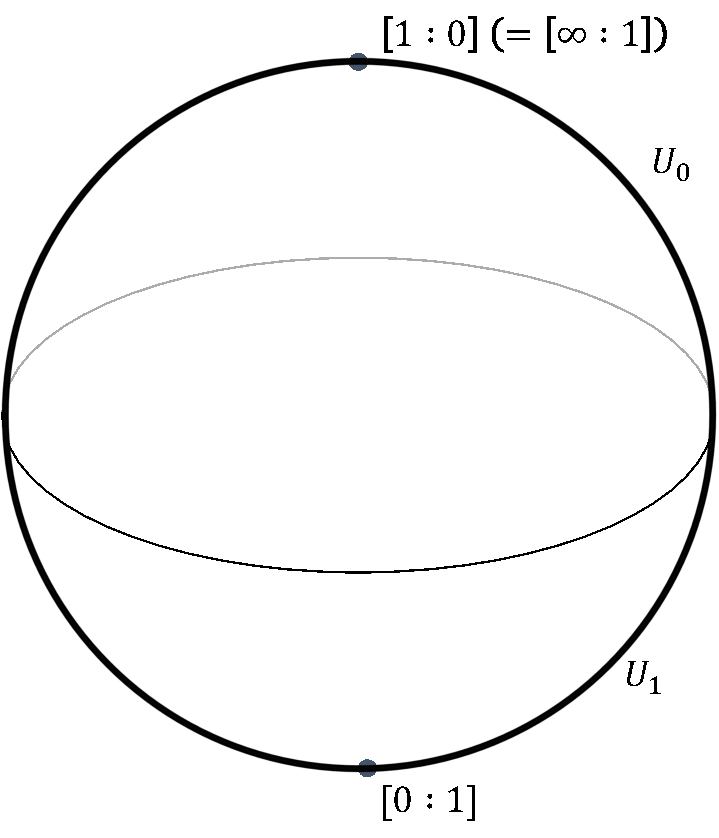
\includegraphics[width=5cm]{fig/riemann-sphere.pdf}
            \centering
        \end{column}
    \end{columns}
\end{frame}
\subsection{複素トーラス}

\begin{frame}
    \frametitle{周期格子}
    \begin{columns}
        \begin{column}{0.45\hsize}
            $\omega_0$, $\omega_1$を$\rr$上一次独立な$0$でない複素数とする.
            このとき,$\cc$の部分加群$\Omega\subset\cc$を
            \begin{equation*}
                \Omega\coloneqq\left\{n_0\omega_0+n_1\omega_1;n_0,n_1\in\zz\right\}
            \end{equation*}
            で定める.$\Omega$を周期格子といい,
            \begin{equation*}
                S\coloneqq\left\{a\omega_0+b\omega_1;0\leqq a,b <1\right\}
            \end{equation*}
            を周期平行四辺形という.
        \end{column}
        \begin{column}{0.45\hsize}
            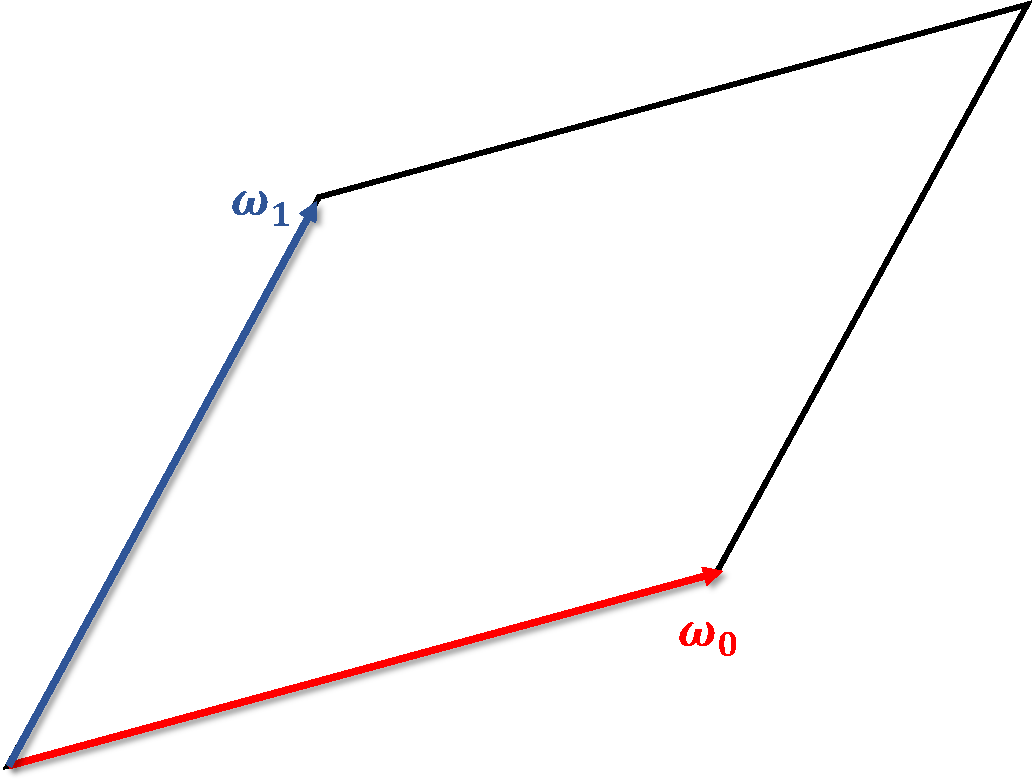
\includegraphics[width=6cm]{fig/lattice.pdf}
            \centering
        \end{column}
    \end{columns}
\end{frame}

\begin{frame}
    \frametitle{複素トーラス}
    \begin{columns}
        \begin{column}{0.45\hsize}
            $E\coloneqq \cc/\Omega$を複素トーラスという.

            $S$と$E$の点は一対一に対応する.

            標準射影$p\colon \cc\to E$による$z\in\cc$の像を$[z]$とかく.
        \end{column}
        \begin{column}{0.45\hsize}
            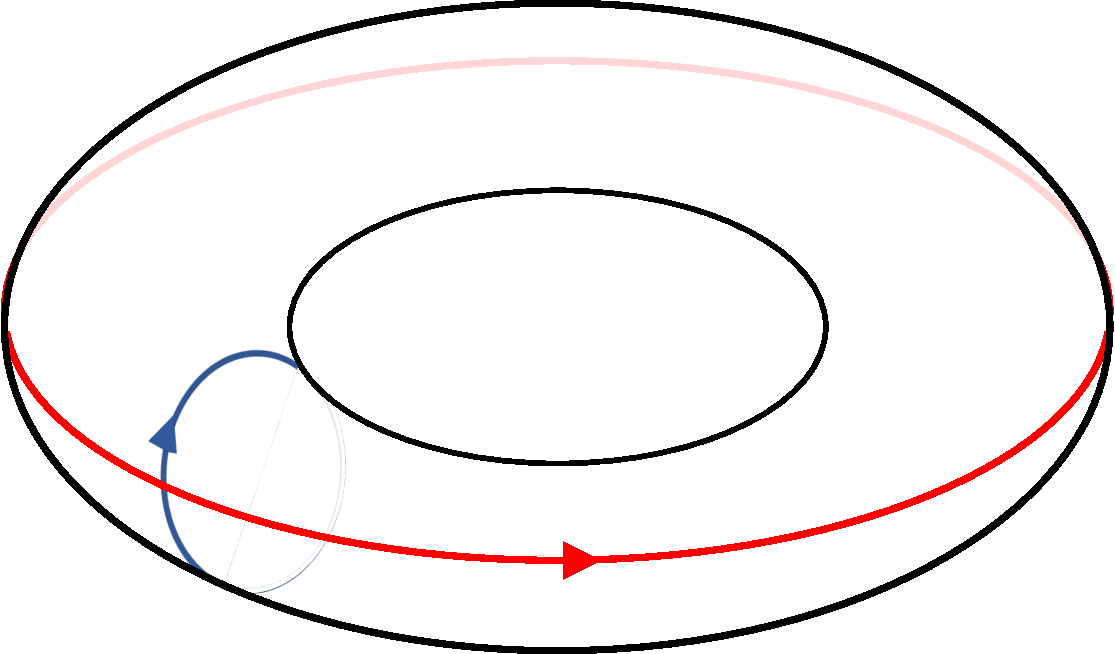
\includegraphics[width=6cm]{fig/torus.pdf}
            \centering
        \end{column}
    \end{columns}
\end{frame}

\begin{frame}
    \frametitle{複素トーラスの複素多様体構造}
        各点$P\in E$の十分小さい開近傍$U_P\subset E$に対し,
        $U_P=p(\UU_x)$となる開集合$\UU_x\subset S$をとる.
        $\dip p^{-1}(U_P)=\underset{\omega\in\Omega}{\bigcup}\UU_x+\omega$である.

        $\omega\in\Omega$を一つ取って
        同相$\pphi_{P,x+\omega}\coloneqq
        \left(\mapres{p}{\UU_x+\omega}\right)^{-1}\colon 
        U_P\to\UU_{x+\omega}$を考える.

        座標変換は平行移動$z\mapsto z+\omega$.


        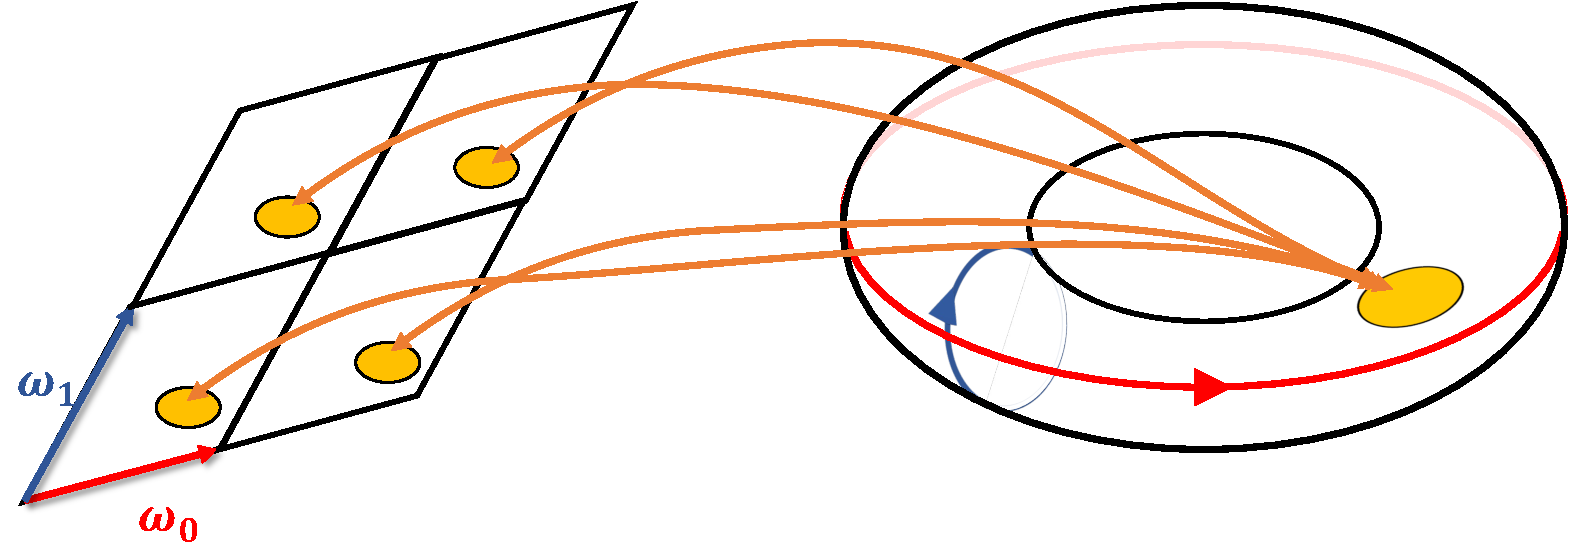
\includegraphics[width=0.7\hsize]{fig/atlas.pdf}
        \centering
\end{frame}

\section{楕円関数}

\begin{frame}
    \frametitle{楕円関数}

    \begin{Definition}
        $\omega_0$, $\omega_1$に対し,
        $\cc$上の有理型関数$f$で
        \begin{equation*}
            f(z+\omega_0)=f(z),\quad f(z+\omega_1)=f(z)
        \end{equation*}
        を満たすものを,$\omega_0$, $\omega_1$を周期とする,
        或は$\Omega$を周期とする
        楕円関数という.
    \end{Definition}

    次の補題がある.
    
    \begin{Lemma}\label{lem:corr}
        商写像$p\colon\cc\to E$の
        引き戻し$p^{\ast}\colon f\mapsto f\circ p$は
        $\{E\text{上の有理型関数}\}$から
        $\{\Omega\text{を周期とする}\cc\text{上の楕円関数}\}$への
        1対1対応を定める.
    \end{Lemma}
\end{frame}


\subsection{楕円関数の例}

\begin{frame}
    \frametitle{Weierstrass の$\wp$関数}

    \begin{Definition}[Weierstrass の$\wp$関数]
        \begin{align*}
            \wp(u)\coloneqq 
            \sum_{\substack{\omega\in\Omega,\\\omega\ne 0}}
            \left(\frac{1}{(u-\omega)^2}-\frac{1}{\omega}\right)
        \end{align*}
        は$\Omega$にのみ2位の極を持つ楕円関数である.
        $\wp$をWeierstrass の$\wp$関数という.
    \end{Definition}

\end{frame}

\section{分岐指数と写像度}

\begin{frame}
    \frametitle{分岐指数}
    \setlength{\baselineskip}{18pt}

    \begin{fact}\label{fact:branch}
        \setlength{\baselineskip}{18pt}
        $X$と$Y$をリーマン面とする.
        $f\colon X\to Y$を定値でない正則写像とする.

        $P\in X$, $Q=f(P)\in Y$とおく.
        
        このとき,$P$のまわりの局所座標$t$と$Q$のまわりの局所座標$s$と
        正の整数$n\geqq 1$で,$f$の
        局所座標表示が$s=t^n$となるものが存在する.
        この$n$は座標の取り方によらない.    
    \end{fact}

\end{frame}

\begin{frame}
    \frametitle{写像度}
    \begin{fact}\label{fact:deg}
        $X$と$Y$をコンパクトリーマン面とし,
        $f\colon X\to Y$を定値でない正則写像とする. 
        このとき,次が成り立つ.
        
        \begin{enumerate}
            \item $\forall Q\in Y$\quad $f^{-1}(Q)\neq\varnothing$, $\#f^{-1}(Q)<\infty$. 
            \item $\#\{f\text{の分岐点}\}<\infty$.
            \item $Q\in Y$, 
            $d(Q)\coloneqq \underset{P\in f^{-1}(Q)}{\sum}e_P$: constant. $\deg f \coloneqq d(Q)$.
            \item $Q\in Y-\{f\text{の分岐点}\}$, $\# f^{-1}(Q)=\deg f$. 
            \item $Q\in \{f\text{の分岐点}\}$, $\# f^{-1}(Q)<\deg f$. 
        \end{enumerate}
        
    \end{fact}

\end{frame}

\begin{frame}
    \frametitle{分岐指数と写像度}

    \begin{definition}[分岐指数]
        上の事実における$n$を$P$における$f$の分岐指数といい,
        $e_P$とかく.
        
        $e_P>1$のとき,$P$を$f$の分岐点という.
    \end{definition}
    \begin{definition}[写像度]
        $d=\deg f$を$f$の写像度といい,$f$を$d$重被覆写像という.
    \end{definition}
\end{frame}

\section{主定理}
\begin{frame}\frametitle{主定理}
    \begin{Theorem}[複素トーラスから射影直線への2重被覆]
        $E$から$\pp^1$への正則射
        \begin{equation*}
            \wp\colon E\to\pp^1;\quad [z]\mapsto [\wp(z);1]    
        \end{equation*}は$\mathrm{4}$点
        \begin{align*}
            [0],
            \left[\frac{\omega_0}{2}\right],
            \left[\frac{\omega_1}{2}\right],
            \left[\frac{\omega_0+\omega_1}{2}\right]
        \end{align*}
        で分岐する$\mathrm{2}$重被覆写像である.
    \end{Theorem}
\end{frame}

\begin{frame}\frametitle{定理の言い換え}
        $P\in \pp^1$に対し,    
    \begin{align*}
        \#\wp^{-1}(P)=
        \begin{cases}
            1\quad ([0],\left[\frac{\omega_0}{2}\right], 
            \left[\frac{\omega_1}{2}\right], 
            \left[\frac{\omega_0+\omega_1}{2}\right]\mapsto P\text{のとき}), \\    
            2\quad (\text{otherwise})
        \end{cases}
    \end{align*}
    ということ.
\end{frame}

\begin{frame}
    \frametitle{証明 (1/2)}
    \setlength{\baselineskip}{18pt}
    $\wp$は$\Omega$にのみ2位の極をもつ楕円関数であったから,
    $[0]$のみに2位の極をもつ$E$上の有理型関数というのと同じである.
    したがって,$\wp^{-1}(\infty)=\{[0]\}$であり,
    写像度に関する事実より,$\deg\wp=2$である.
    いま,$\wp$は偶関数なので,$[a]\in E$に対し,
    $\wp([a])=\wp([-a])$が成り立つ.
    $[a]$が$E$の2分点でなければ,$[a]\neq[-a]$である.
    $\deg\wp=2$なので,
    このとき,$\wp^{-1}(\wp([a]))=\{[a],[-a]\}$と確定する.
\end{frame}

\begin{frame}
    \frametitle{証明 (2/2)}
    \setlength{\baselineskip}{18pt}
%    $\fracinline{\omega_0}/{2}$
    $[\omega_0/2]$の近傍で$\wp$を局所座標表示する.
    $\wp$は$\omega_0$を周期にもつ偶関数なので
    $\wp(-z)=\wp(z)=\wp(z+\omega_0)$をみたす.
    両辺を微分して,
    $-\wp'(-z)=\wp'(z+\omega_0)$となるが,$z=-\omega_0/2$のとき,
    $-\wp'(\omega_0/2)=\wp'(\omega_0/2)$となる.
    したがって,$\wp'(\omega_0/2)=0$となる.
    よって,$\wp(z)$の$\omega_0/2$のまわりでの
    展開における1次の項の係数は0である.
    したがって,$e_{[\omega_0/2]}>1$であり,
    $[\omega_0/2]$は$\wp$の分岐点である.

    $[\omega_1/2]$と$[(\omega_0+\omega_1)/2]$についても同様に,
    $e_{[\omega_1/2]}>1$, $e_{[(\omega_0+\omega_1)/2]}>1$となるので,
    $\wp$は$E$の2分点で分岐する2重被覆であることが示せた.

\end{frame}
    

\begin{comment}
    \begin{frame}\frametitle{同値関係の幾何的イメージ}
    %\scalebox{0.8}{
    \begin{tikzpicture}
        \draw[>=stealth,semithick] (-2,0)--(3,0); %x軸
        \draw[>=stealth,semithick] (0,-2)--(0,4); %y軸
        \draw (0,0)node[below right]{O}; %原点
        \draw[thick, domain=-2:3] plot(\x,{0.5*\x});
        \draw[thick, domain=-1.:2] plot(\x,2*\x);
        \fill[black!20] (1.5,3) rectangle (2.5,1.25); %四角2U
        \draw[line width = 0.5pt] (1.5,3) rectangle (2.5,1.25); %四角2U
        \draw (2.5,1.25)node[below]{$2U$}; %点(2.5,1.25)
        \fill[black!20] (1,2) rectangle (1.66,0.83); %四角Uずらし
        \draw[line width = 0.5pt] (1,2) rectangle (1.66,0.83); %四角Uずらし
        \fill[black!40] (0.75,1.5) rectangle (1.25,0.625); %四角U
        \draw[line width = 0.5pt] (0.75,1.5) rectangle (1.25,0.625); %四角U
        \draw (0.75,1.5)node[left]{$U$}; %点(2.5,1.25)\draw[line width=1pt] (0.75,1.5) rectangle (1.25,0.625); %四角
        \fill[black!20] (-0.75,-1.5) rectangle (-1.25,-0.625); %四角-U
        \draw[line width = 0.5pt] (-0.75,-1.5) rectangle (-1.25,-0.625); %四角-U
        \fill[black!20] (-1,-2) rectangle (-1.66,-0.83); %四角-U
        \draw[line width = 0.5pt] (-1,-2) rectangle (-1.66,-0.83); %四角-U
        \draw (-0.75,-1.5)node[right]{$-U$}; %点(2.5,1.25)
        \fill[black!20] (0.375,0.75) rectangle (0.625,0.3125); %四角(1/2)U
        \draw[line width = 0.5pt] (0.375,0.75) rectangle (0.625,0.3125); %四角(1/2)U
        \draw (0.625,0.2)node[right]{$(1/2)U$}; %点(2.5,1.25)
        \draw[very thick, domain=-2.:3] plot(\x,{0.8*\x});
        %\draw[very thick, domain=-1.7:2.7] plot(\x,{1.3*\x});
        \draw (1.8,3.6)node[right]{$U$を通る直線の上端};
        \draw (3,2.4)node[right]{$U$を通る直線};
        \draw (3,1.5)node[right]{$U$を通る直線の下端};
    \end{tikzpicture}
    \centering
    %}
        %\caption{商写像の逆像1}
\end{frame}

\end{comment}

\section{参考文献}

\begin{frame}[allowframebreaks]{参考文献}
    \begin{thebibliography}{Og02}\beamertemplatetextbibitems
        \bibitem[Og02]{1} 小木曽啓示, 
        『代数曲線論』, 朝倉書店, 2002.
    \end{thebibliography}
\end{frame}

\begin{comment}
\begin{frame}[noframenumbering]
aaa
\end{frame}
\end{comment}

\end{document}